% This must be in the first 5 lines to tell arXiv to use pdfLaTeX, which is strongly recommended.
\pdfoutput=1
% In particular, the hyperref package requires pdfLaTeX in order to break URLs across lines.

\documentclass[11pt]{article}

% Remove the "review" option to generate the final version.
\usepackage[]{acl}

% Standard package includes
\usepackage{times}
\usepackage{latexsym}
\usepackage{graphicx}
\usepackage{amsmath}
\usepackage{float}
\usepackage[export]{adjustbox} 

% For proper rendering and hyphenation of words containing Latin characters (including in bib files)
\usepackage[T1]{fontenc}
% For Vietnamese characters
% \usepackage[T5]{fontenc}
% See https://www.latex-project.org/help/documentation/encguide.pdf for other character sets

% This assumes your files are encoded as UTF8
\usepackage[utf8]{inputenc}

% This is not strictly necessary, and may be commented out,
% but it will improve the layout of the manuscript,
% and will typically save some space.
\usepackage{microtype}

% If the title and author information does not fit in the area allocated, uncomment the following
%
%\setlength\titlebox{<dim>}
%
% and set <dim> to something 5cm or larger.

\title{DD-TIG at Constraint@ACL2022: Multimodal Understanding and Reasoning for Role Labeling of Entities in Hateful Memes}

% Author information can be set in various styles:
% For several authors from the same institution:
% \author{Author 1 \and ... \and Author n \\
%         Address line \\ ... \\ Address line}
% if the names do not fit well on one line use
%         Author 1 \\ {\bf Author 2} \\ ... \\ {\bf Author n} \\
% For authors from different institutions:
% \author{Author 1 \\ Address line \\  ... \\ Address line
%         \And  ... \And
%         Author n \\ Address line \\ ... \\ Address line}
% To start a seperate ``row'' of authors use \AND, as in
% \author{Author 1 \\ Address line \\  ... \\ Address line
%         \AND
%         Author 2 \\ Address line \\ ... \\ Address line \And
%         Author 3 \\ Address line \\ ... \\ Address line}

 \author{Ziming Zhou$^2$, Han Zhao$^1$, Jingjing Dong$^2$, Jun Gao$^1$, Xiaolong Liu$^1$\\
 $^1$DD-TIG\\
$^2$Peking University\\
\texttt{\{zhaohan,gaojun\_i,xlongliu\}@didiglobal.com} \\
\texttt{\{zhouziming,djj\}@stu.pku.edu.cn} \\
}


\begin{document}
\maketitle
\begin{abstract}
The memes serve as an important tool in online communication, whereas some hateful memes endanger cyberspace by attacking certain people or subjects. Recent studies address hateful memes detection while further understanding of relationships of entities in memes remains unexplored. This paper presents our work at the Constraint@ACL2022 Shared Task: Hero, Villain and Victim: Dissecting harmful memes for semantic role labelling of entities. In particular, we propose our approach utilizing transformer-based multimodal models through a visual commonsense reasoning (VCR) method with data augmentation, continual pretraining, loss re-weighting, and ensemble learning. We describe the models used, the ways of preprocessing and experiments implementation. As a result, our best model achieves the Macro F1-score of 54.707 on the test set of this shared task\footnote{\url{https://github.com/zjl123001/DD-TIG-Constraint}}. 
\end{abstract}

\section{Introduction}

Memes are getting popular as a communication tool on social media platforms for expressions of opinions and emotions, conveying a subtle message through multimodal information from both images and texts. However, memes are increasingly abused to spread hate instigate social unrest and therefore seem to be a new form of expression of hate speech on online platforms \citep{bhattacharya2019social}.

Automatic hateful memes detection is difficult since it primarily requires context and external knowledge to understand online speech, which sometimes can be very short and contains nuanced meaning \citep{pramanick2021detecting}. A new type of challenging task has been introduced by The Hateful Memes Challenge \citep{kiela2020hateful} proposed by Facebook AI to leverage machine learning models to address hateful memes detection problems, which can only be solved by joint reasoning and understanding of visual and textual information \citep{zhu2020enhance}. 

In previous studies, researchers focus on binary classification problems, labelling a meme as hateful or non-hateful based on image and text features \citep{afridi2020multimodal}. Moreover, the relationships of entities in memes remain unexplored, and the task of role labelling of entities in hateful memes can be more sophisticated.

The Constraint@ACL2022 Shared Task: Hero, Villain and Victim: Dissecting harmful memes for semantic role labelling of entities offers us a perspective on this issue \citep{sharma2022report}. This task aims to promote the detection and classification of glorified, vilified or victimized entities within a meme. The shared dataset concerns memes from US Politics domains and Covid-19. Covid-19-related online hostile content especially demands to be detected as early as possible after their appearance on social media. 

In this paper, we present our work on this task. Specifically, mainstream multimodal models of transformer-based architecture are applied through a visual commonsense reasoning (VCR) method, with the leverage of continual pretraining to fit models with our dataset. Then, data augmentation and loss re-weighting are implemented to improve the performance of models. The predictions from variant models are combined in a machine learning method to produce final results. 



\section{Related Work}

Hateful memes understanding and reasoning is a vision and language task. Current state-of-the-art Vision-Language machine learning models are based on the transformer architecture \citep{vaswani2017attention}. Multimodal models learn the joint visual and textual representations through self-supervised learning that utilize large-scale unlabelled data to conduct auxiliary tasks \citep{chen2022vlp}, including masked language modelling based on randomly-masked sub-words, masked region prediction and image-text matching. Among these models, there are two prevalent approaches: single-stream and dual-stream \citep{du2022survey}. 

In single-stream architecture, the representations of two modalities are learned by a single transformer encoder. Particularly, the text embeddings $ L  = \{w_1, w_2, w_3, \cdots, w_l\} $ and image features $V = \{o_1, o_2,o_3, \cdots , o_k\}$ are concatenated together as $X = \{ L \mathbin\Vert  V \} $, added some special embeddings to indicate position and modalities, and fed into a transformer-based encoder.

There are many implementations in single-stream models, such as VisualBERT \citep{li2019visualbert}, UNITER \citep{chen2020uniter}, OSCAR 
\citep{li2020oscar}.

In dual-stream models, the image and text features are first sent to two independent encoders. Then two features are separately fed into cross-modal transformer layers, where the query vectors are from one modality while the key and value vectors are from another. They are responsible for exchanging the information and aligning the semantics between the two modalities $L$ and $V$. The formula of cross-modal transformer layers is represented as follows.

\begin{small}
\begin{equation}
L^m_i = CrossAtt_{L-V} (L^{m-1}_i,\{ V^{m-1}_1, \cdots, V^{m-1}_k \} )
\end{equation}
\begin{equation}
V^m_i = CrossAtt_{V-L} (V^{m-1}_i,\{ L^{m-1}_1, \cdots, L^{m-1}_l \} )
\end{equation}
\end{small}
where $m$ is the $m^{th}$ cross-attention layer, $k$ is the number of visual tokens, and $l$ is the length of text tokens.

Following each cross-attention layer, there is also a layer computing the self-attention of each modality independently. Features are combined at the end of the model. 

Several dual-stream models have been proposed in former studies, such as LXMERT \citep{tan2019lxmert}, ERNIE-Vil \citep{yu2020ernie}, DeVLBERT \citep{zhang2020devlbert}, VilBERT \citep{lu2019vilbert}, 

\section{Task Definition}

Given the image and transcribed text of a meme, the role of a certain entity in this meme will be determined as hero, villain, victim or other, which can be interpreted as a multi-class classification task.

\begin{itemize}
\item \textbf{Input:} a meme image $V$, text transcriptions $L$, a entity $E$

\item \textbf{Output:} $y \in \{hero, villain, victim, other\}$

\end{itemize}

The official evaluation measure for the shared task is the macro-F1 score for the multi-class classification.

\section{Data Composition}

The dataset provided in this task is a combination of memes from Covid-19 and US Politics domain. Every sample in the train and validation set contains an image, a transcription of texts and a list of entities with annotated labels. The shared task organizers provide the definitions for each class \footnote{\url{https://codalab.lisn.upsaclay.fr/competitions/906}}:

\begin{itemize}
\item \textbf{Hero:} the entity is presented in a positive light, glorified for its actions.

\item \textbf{Villain:} the entity is portrayed negatively, e.g., in an association with adverse traits like wickedness, cruelty, hypocrisy, etc.

\item \textbf{Victim:} the entity is portrayed as suffering the negative impact of someone else's actions or conveyed implicitly within the meme.

\item \textbf{Other:} the entity is not a hero, a villain, or a victim.

\end{itemize}

We present the distribution of entities' roles in Table \ref{dataset-table}.


\begin{table}[h]
\centering
\begin{tabular}{lllll}
\hline
\multicolumn{5}{c}{\textbf{Covid-19}}                                                \\ \hline
               & \textbf{Hero} & \textbf{Villain} & \textbf{Victim} & \textbf{Other} \\
\textbf{Train} & 190           & 662              & 360             & 6022           \\
\textbf{Val}   & 20            & 81               & 48              & 674            \\
\textbf{Test}  & 21            & 124              & 58              & 1087           \\ \hline
\multicolumn{5}{c}{\textbf{US Politics}}                                             \\ \hline
\textbf{}      & \textbf{Hero} & \textbf{Villain} & \textbf{Victim} & \textbf{Other} \\
\textbf{Train} & 285           & 1765             & 550             & 7680           \\
\textbf{Val}   & 34            & 224              & 73              & 915            \\
\textbf{Test}  & 31            & 226              & 56              & 830           \\ \hline   
\end{tabular}
\caption{\label{dataset-table}Numbers of sample for each role label in Covid-19 and US Politics domain }

\end{table}

There is a considerable imbalance in the distribution of entities' roles where the “other” class accounts for more than 80 percent of the whole dataset. Meanwhile, the distribution of entities' frequency also shows a disparity. We present some most frequent entities with their roles distribution in Figure \ref{Entitites}.

\begin{figure}[h]
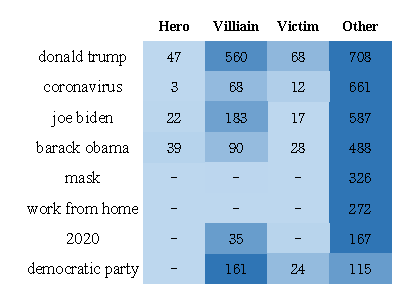
\includegraphics[width=0.45\textwidth]{Entitites.pdf}
\caption{\label{Entitites}Roles distribution of most frequent entities}

\end{figure}


\section{System Descriptions}

\begin{figure*}[h]
\centering
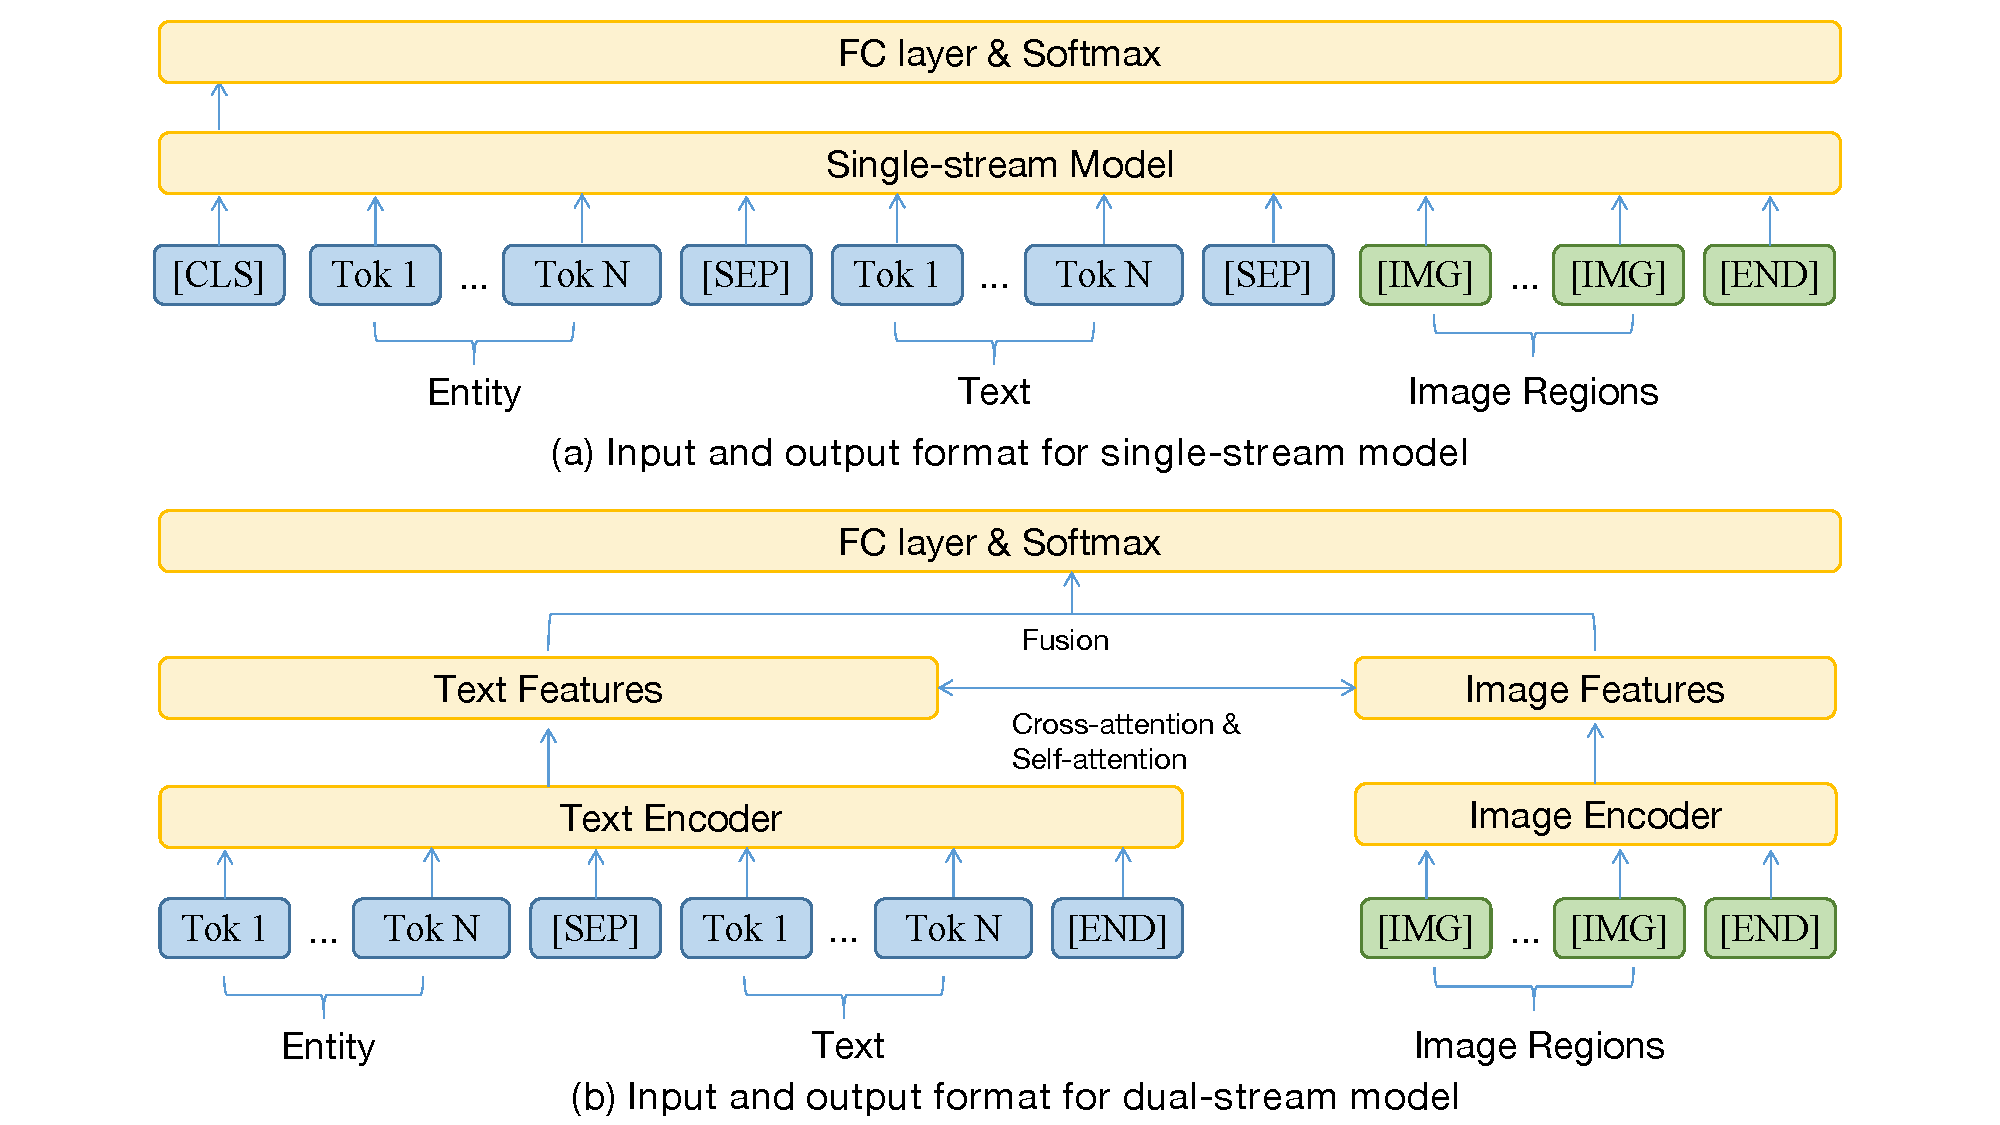
\includegraphics[width=\textwidth]{V.pdf}
\caption{\label{VCR}The input and output format of our system}
\end{figure*}


\subsection{Preparation}


For visual feature preprocessing, we use the pretrained Mask-RCNN model provided in the detectron2 framework\footnote{\url{https://github.com/facebookresearch/detectron2}} to obtain the object detection based region feature embedding $V = [o_1, o_2, \cdots , o_k]$ of images. Detectron2 is proposed by Facebook AI with state-of-the-art detection and segmentation algorithms. Specifically, 50 boxes of 2048 dimensions region-based image features are extracted for every meme. For the text transcriptions, we make the content lower-case and remove punctuation and stopwords with NLTK library \citep{loper2002nltk}.



\subsection{Vision and Language Models}

Four mainstream multimodal models of VL transformer architectures are applied in this work, namely: VisualBERT, UNITER, OSCAR, and ERNIE-Vil. 

\paragraph{VisualBERT} \citep{li2019visualbert}, known as the first image-text pre-training model, uses the visual features extracted by Faster R-CNN, concatenates the visual features and textual embeddings, and then feeds the concatenated features to a single transformer initialled by BERT.

\paragraph{UNITER} \citep{chen2020uniter} learns contextualized joint representation of both visual and textual modalities through local alignment in the reconstruction of masked tokens/regions across modalities, powering heterogeneous downstream V+L tasks with joint multimodal embeddings.

\paragraph{OSCAR}\citep{li2020oscar}, instead of simply using image-text pair, adds object tags detected from the image and represent the image-text pair as a <Word, Tag, Image> triple to help the fusion encoder better align different modalities.

\paragraph{ERNIE-Vil} \citep{yu2020ernie}, as a typical dual-stream model, enhances the model with the application of scene utilizing scene graphs of visual scenes, which can learn the joint representations characterizing the alignments of the detailed semantics across vision and language. 

\paragraph{} For domain adaptation, we carry out continual pretraining on our dataset to reduce the distribution gap between the pretraining dataset and our memes dataset. Masked Language Modeling (MLM) pretraining task is taken on pretraining VisualBERT-large, UNITER-large, and OSCAR-large model.




\subsection{VCR Implementation}

Visual Commonsense Reasoning (VCR) focuses on a higher-order cognitive and commonsense understanding of relationships of the visual components in the image \citep{zellers2019recognition}. Former studies take a question, answer choices and an image into models to predict the right answer as a multi-class classification problem \citep{su2019vl}. We modify this method's input and output format to conduct our experiments. 

As can be seen in Figure \ref{VCR}, we concatenate the given entity and text tokens as the textual input with a separate token $[SEP]$, while different segment embedding will be added respectively to indicate their states. Then, textual input and visual will be concatenated in the single-stream model like VisualBERT. They would be separately sent into encoders in the dual-stream model like ERNIE-Vil. In the single-stream model, the final output feature of $[CLS]$ element is taken. In the dual-stream model, textual and visual features are fused through sum or multiplication. Then, features are fed to a linear layer with softmax to predict the role of the given entity. 

The final objective is to minimize the cross-entropy (CE) loss between the predicted distribution and the targeted role category, which can be formally defined as:

\begin{small}
\begin{equation}
    p(x) = \frac{exp(g(x)_i)}{\sum_{j=1}^N exp(g(x)_j)}
\end{equation}

\begin{equation}
    L = - \sum log{p(x)} \cdot y
\end{equation}
\end{small}

where $g(x)$ is the output of the FC layer and $N$ is the number of labels.

\subsection{Loss Re-weighting}
A loss re-weighting strategy has been applied in our experiment since the "other" class accounts for the overwhelming majority of entries in samples, while hero, villain, and victim roles shall be stressed. Thus, our new loss function is defined as follows:


\begin{equation}
L = - \sum \alpha  \cdot  \log{p(x)}
\end{equation}
 \begin{equation}
  \alpha = \begin{cases} \alpha_{neg} & y = other \\ \alpha_{pos} & else\\ \end{cases} 
 \end{equation}
where $\alpha_{neg}$ and $\alpha_{pos}$ are the weights for the "other" role and "non-other" role respectively as $\alpha_{neg}$ < $\alpha_{pos}$ and $\alpha_{neg} + \alpha_{pos} = 1$. 

\begin{table*}[h]
\centering
\begin{tabular}{cll}
\hline
\multicolumn{1}{l}{\textbf{Source}}         & \textbf{Model}   & \textbf{Macro F1-score} \\ 
\hline
\multirow{Original model} & VisualBERT-large & 47.8                    \\
                                            & UNITER-large     & 48.8                    \\
                                            & OSCAR-large      & 48.5                    \\
                                            & ERNIE-Vil-large  & 50.9                    \\ \hline
\multirow{Continual pretrained model} & VisualBERT-large & 48.2                    \\
                                            & UNITER-large     & 49.9                    \\
                                            & OSCAR-large      & 49.2                    \\ \hline
\multicolumn{1}{l}{}                        & Ensemble         & \textbf{54.7}                    \\ \hline
\end{tabular}
\caption{\label{result} Results of models in our systems }
\end{table*}

\subsection{Data Augmentation}

We adopt the data augmentation with the back-translation strategy. Specifically, the provided text of each meme is paraphrased with Baidu translation API: English-Chinese-English and English-French-English. Diverse sentences are produced for each meme to enrich our dataset.


\subsection{Ensemble Learning}

We train these four base models with different seeds to produce a total of 16 models. The predicted scores on validation set are generated by all models. Then, a SVM model is trained with the predictions and true labels. In the testing phase, the predictions on the test set are fed into the trained SVM model to make final ensemble predictions.

\subsection{Experimental Setting}
For continual pretraining on VisualBERT, OSCAR, and UNITER, each word in the text transcriptions is randomly masked at a probability of 15 percent. The final output feature corresponding to the masked word is fed into a classifier over the whole vocabulary, driven by softmax cross-entropy loss.

We finetune all models with a focal loss \citep{lin2017focal} and a batch size of 16. The max sequence length is set at 256. The Adam optimizer is used with a learning rate of 1e-5 and 10 percent linear warm-up steps. VisualBERT, OSCAR, and UNITER are trained for 10 epochs and ERNIE-Vil models are trained for 10000 steps. The weights with the best scores on the validation set are saved and used for inference on the test set.




\section{Results and Discussion}

In Table \ref{result}, we present the results of our experiments in a step by step manner. We started with finetuning base models provided by original authors. Then, VisualBERT-large, UNITER-large, and OSCAR-large models are pretrained on our dataset with MLM task and finetuned on our task. After that, ensemble learning is implemented to combine results of various models. We evaluate our models using official metrics Macro F1-score on test set.

ERNIE-Vil has been the SoTA model on the multimodal task leaderboard and in this task it also achieves competitive performance at 50.9 on the test set without further continual pretraining, which outperforms all the single-stream models by over 2 in Macro F1-score. We consider that through incorporating structured knowledge obtained from scene graphs during cross-modal pre-training, ERNIE-Vil learns more knowledge which benefits the downstream task. 

Meanwhile, VisualBERT-large, UNITER-large, and OSCAR-large models shows improvements in performance through continual pretraining, which can be interpreted as domain adaptation on our dataset. 

Ensemble learning remarkably raises our score by 3.5 than the best single model, which achieves the best score for our submission in this task. 

\subsection{Error Analysis}
A classification report is presented in table \ref{report}, which allows us to do further assessments on our system.

\begin{table}[h]
\centering
\resizebox{7cm}{!}{
\begin{tabular}{lllll}
\hline
          & \multicolumn{1}{c}{\textbf{precision}} & \multicolumn{1}{c}{\textbf{recall}} & \multicolumn{1}{c}{\textbf{f1-score}} & \multicolumn{1}{c}{\textbf{support}} \\ \hline
Hero      & 0.31                                   & 0.33                                & 0.32                                  & 52                                   \\
Villain   & 0.55                                   & 0.50                                & 0.52                                  & 350                                  \\
Victim    & 0.44                                   & 0.41                                & 0.43                                  & 114                                  \\
Other     & 0.88                                   & 0.89                                & 0.89                                  & 1917                                 \\ \hline
Macro-avg & 0.54                                   & 0.53                                & 0.54                                  & 2433                                 \\ \hline
\end{tabular}}
\caption{\label{report} An classification report for our final submission}
\end{table}


Our system has a relatively poor performance on the class Hero. On the one hand, we interpret it as a lack of sample of this class in the training set. It is insufficient for our model to learn the features of this class. On the other hand, through observing bad cases, we find some memes need considerable external knowledge about history and politics, which can even be challenging for human beings to comprehend and do classification.


\subsection{Future Directions}

In our experiment, we use an End2End solution to do roles classification, concatenating the entity with input sequence as a <entity, text, image> triplet. However, we do not directly point out the entity's corresponding region in the image. Some other researchers \citep{li2020oscar} have discussed this problem: it is naturally weakly-supervised learning since there are no explicitly labelled alignments between regions or objects in an image and words or phrases in the text. We hypothesize that our model can not align some unusual entities correctly with its image and text. Moreover, comprehending a meme in the political domain heavily relies on knowledge, while the size of the whole dataset is relatively small, so our continual pretraining on a task-specific dataset is far from sufficient. There are two directions for further development of our system on this issue. On the one hand, more in-domain data can be incorporated to enlarge the dataset. On the other hand, knowledge-based models or external knowledge sources can be introduced to help the model understand the background and reason the relations of entities.




\section{Conclusion}

In this paper, we have exploited a VCR approach to tackle the role labelling of entities in hateful memes, which is a novel task in multimodal understanding and reasoning. Four popular transformer-based multimodal models, VisualBERT, UNITER, OSCAR, and ERNIE-Vil are applied as base models while strategies like loss re-weighting and data augmentation are implemented during the training of models. Then, continual pretraining is taken for domain adaptation and achieves better performance. Ensemble learning of variant models achieves the impressive Macro F1-score of 0.5470 on the final (unseen) test set.


% Entries for the entire Anthology, followed by custom entries
\bibliography{anthology,custom}
\bibliographystyle{acl_natbib}


\end{document}
